\section{Multivariate normal distribution ($N(\mu, \Sigma)$)}

\begin{figure}[H]
    \centering
    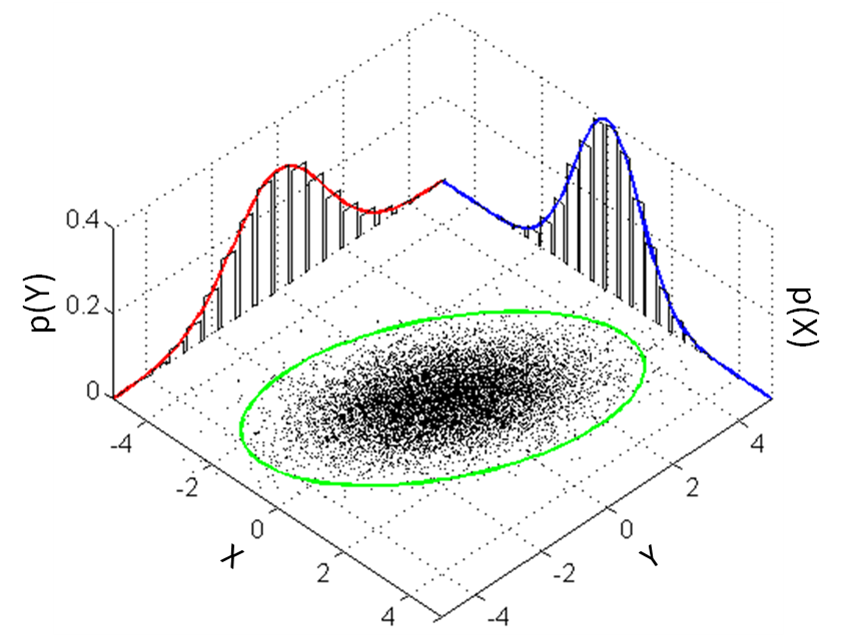
\includegraphics[
        width=\linewidth,
        height=6cm,
        keepaspectratio,
    ]{images/distributions/MultivariateNormal-pdf.png}
    \caption{Multivariate normal distribution: PDF \cite{wiki/Multivariate_normal_distribution}}
\end{figure}


\subsection{PDF}

\begin{enumerate}
    \item
    $
        \mathcal{N}(\bm{x}|\bm{\mu}, \bm{\Sigma})
        = (2\pi)^{-D/2} \dabs{\bm{\Sigma}}^{-1/2} \,
        \exp\dParenBrac{
            -\dfrac{1}{2}
            (\bm{x} - \bm{\mu})^\top \bm{\Sigma}^{-1} (\bm{x} - \bm{\mu})
        }
    $
    \hfill \cite{ml/book/Pattern-Recognition-And-Machine-Learning/Christopher-M-Bishop}
    \\[0.2cm]
    .\hfill
    $\bm{x}, \bm{\mu} \in \mbbR^D$
    \hfill
    $\bm{\Sigma} \in \mbbR^{D \times D}$
    \hfill
    $\dabs{\bm{\Sigma}} = \det(\bm{\Sigma}) \in \mbbR$
    \hfill \cite{ml/book/Pattern-Recognition-And-Machine-Learning/Christopher-M-Bishop}

    \item when $X$ and $Y$ are marginally normally distributed, there are different ways of creating dependencies between $X$ and $Y$ that are different from the bivariate PDF
    \hfill \cite{statistics/book/Statistics-for-Data-Scientists/Maurits-Kaptein}
    \\
    Even if two random variables $X$ and $Y$ each individually follow a normal distribution (i.e., their marginals are normal), the way in which they are dependent or correlated can vary.
    That is, their joint distribution doesn't have to be the bivariate normal distribution
    \hfill \cite{common/online/chatgpt}
\end{enumerate}



\subsection{Bivariate Normal Distributions}

\begin{enumerate}[series=binvar-normal]
    \item PDF:
    $
        f (x, y)
        = \dfrac{1}{ 2\pi\sigma_X \sigma_Y \sqrt{1 - \rho^2} }
        \exp \dParenBrac{
            - \dfrac{z^2_1 - 2\rho z_1z_2 + z^2_2 }{2(1 - \rho^2)}
        }
    $
    \hfill \cite{statistics/book/Statistics-for-Data-Scientists/Maurits-Kaptein}
    \begin{enumerate}
        \item $z_1 = \dfrac{x - \mu_X}{\sigma_X}$: standardized normal variable for $X$
        \hfill \cite{statistics/book/Statistics-for-Data-Scientists/Maurits-Kaptein}

        \item $z_2 = \dfrac{y - \mu_Y}{\sigma_Y}$: standardized normal variable for $Y$
        \hfill \cite{statistics/book/Statistics-for-Data-Scientists/Maurits-Kaptein}

        \item $\rho$: \textbf{correlation coefficient} and is contained within the interval $[-1, 1]$.
        \hfill \cite{statistics/book/Statistics-for-Data-Scientists/Maurits-Kaptein}

        \item When $\rho = 0$, the normal random variables $X$ and $Y$ are \textbf{independent}
        \hfill \cite{statistics/book/Statistics-for-Data-Scientists/Maurits-Kaptein}

        \item when $\rho \neq 0$, the normal random variables $X$ and $Y$ are \textbf{dependent}
        \hfill \cite{statistics/book/Statistics-for-Data-Scientists/Maurits-Kaptein}
    \end{enumerate}

    \item
    $
        \begin{aligned}
            \tCov[X, Y]
            & = \mbbE[(X - \mu _X )(Y - \mu _Y )]
            = \sigma _X \sigma _Y \mbbE[Z_1 Z_2] \\
            &= \sigma _X \sigma _Y \dint^\infty_{-\infty} \dint^\infty_{-\infty} z_1z_2 \dfrac{1}{2\pi (1-\rho^2)} \exp \dParenBrac{ - \dfrac{z^2_1-2\rho z_1 z_2+z^2_2} {2(1-\rho^2)} } dz_1\ dz_2\\
            &= \sigma _X \sigma _Y \dint^\infty_{-\infty} z_2 \dfrac{1}{\sqrt{2\pi}}  \exp \dParenBrac{ - \dfrac{z^2_2} {2} } \dint^\infty_{-\infty} z_1 \dfrac{1}{\sqrt{2\pi (1-\rho^2)}} \exp \dParenBrac{ - \dfrac{(z_1-\rho z_2)^2 }{2(1-\rho^2)} } dz_1\ dz_2 \\
            &= \sigma_X \sigma_Y \dint^\infty_{-\infty} \rho z^2_2 \dfrac{1}{\sqrt{2\pi}}  \exp \dParenBrac{ - \dfrac{z^2_2}{ 2} } dz_2
            = \rho \sigma_X \sigma_Y
        \end{aligned}
    $
    \hfill \cite{statistics/book/Statistics-for-Data-Scientists/Maurits-Kaptein}

    \item Consider a Gaussian distributed random variable $X \sim \mathcal{N}(\bm{\mu }, \bm{\Sigma})$. 
    For a given matrix $\bm{A}$ of appropriate shape, let $Y$ be a random variable such that $\bm{y} = \bm{Ax}$ is a transformed version of $\bm{x}$. 
    We can compute the mean of $\bm{y}$ by exploiting that the expectation is a linear operator as follows:
    \hfill \cite{mfml/book/mml/Deisenroth-Faisal-Ong}
    \\[0.2cm]
    .\hfill
    $
        \mbbE[\bm{y}] = \mbbE[\bm{Ax}] = \bm{A}\mbbE[\bm{x}] = \bm{A\mu }
    $
    \hfill \cite{mfml/book/mml/Deisenroth-Faisal-Ong}
    \\[0.2cm]
    the variance of $\bm{y}$: $ \mbbV[\bm{y}] = \mbbV[\bm{Ax}] = \bm{A}\mbbV[\bm{x}]\bm{A}^\top = \bm{A\Sigma A}^\top $
    \hfill \cite{mfml/book/mml/Deisenroth-Faisal-Ong}
    \\[0.2cm]
    the random variable $\bm{y}$ is distributed according to $ P(\bm{y}) = \mathcal{N} (\bm{y} | \bm{A\mu}, \bm{A\Sigma A}^\top) $
    \hfill \cite{mfml/book/mml/Deisenroth-Faisal-Ong}
    \\[0.2cm]
    $\bm{x}$ is a linear transformation of $\bm{y}$, and we obtain:
    \hfill \cite{mfml/book/mml/Deisenroth-Faisal-Ong}
    \\[0.2cm]
    .\hfill
    $
        P(\bm{x}) = \mathcal{N} (\bm{x} | (\bm{A}^\top\bm{A})^{-1}\bm{A}^\top \bm{y}, \ (\bm{A}^\top\bm{A})^{-1}\bm{A}^\top \bm{\Sigma A}(\bm{A}^\top\bm{A})^{-1})
    $
    \hfill \cite{mfml/book/mml/Deisenroth-Faisal-Ong}
    

    \item The distribution function of any linear combination of $X$ and $Y$ , say $a X + bY$ , has a normal distribution function with mean $\mu = a\mu_X + b\mu_Y$ and variance $\sigma ^2 = a^2\sigma ^2_X + 2ab\rho \sigma _X \sigma _Y + b^2\sigma ^2_Y$ .
    \hfill \cite{statistics/book/Statistics-for-Data-Scientists/Maurits-Kaptein}

    \item Pearson’s Correlation Coefficient: $\rho_P = CORR(X, Y) = \rho$
    \hfill \cite{statistics/book/Statistics-for-Data-Scientists/Maurits-Kaptein}

    \item Kendall’s tau: $\tau_K = \dfrac{2 \arcsin(\rho)}{\pi}$
    \hfill \cite{statistics/book/Statistics-for-Data-Scientists/Maurits-Kaptein}

    \item Spearman’s rho correlation: $\rho_S = \dfrac{6}{\pi}\arcsin\dParenBrac{\dfrac{\rho}{2}}$
    \hfill \cite{statistics/book/Statistics-for-Data-Scientists/Maurits-Kaptein}

    \item if $\rho_P = 0$ and the pairs $(X_i , Y_i )$ are i.i.d. bivariate normally distributed, the distribution function of \textbf{Pearson’s Correlation Coefficient estimator} $r_P$ is related to the $t$-distribution.
    \hfill \cite{statistics/book/Statistics-for-Data-Scientists/Maurits-Kaptein}
    \begin{enumerate}
        \item  CDF of $\dfrac{r_P \sqrt{n - 2}}{\sqrt{1 - r_P}}$ has the CDF of a t-distribution with $n - 2$ degrees of freedom.
        \hfill \cite{statistics/book/Statistics-for-Data-Scientists/Maurits-Kaptein}

    \end{enumerate}

    \item  For any value of $\rho_P$, but still assuming that the pairs $(X_i , Y_i )$ are bivariate normally distributed, $z_{r_P} = 0.5[\log(1 + r_P ) - \log(1 - r_P )]$ is approximately normally distributed with mean $0.5[\log(1 + \rho_P ) - \log(1 - \rho_P )]$ and variance $\dfrac{1}{n - 3}$.
    \hfill \cite{statistics/book/Statistics-for-Data-Scientists/Maurits-Kaptein}
    \\
    Transformation of $r_P \mapsto z_{r_P}$ is called \textbf{Fisher z-transformation}.
    \hfill \cite{statistics/book/Statistics-for-Data-Scientists/Maurits-Kaptein, common/online/chatgpt}

    \item Under the assumption of normality, it is common to use the Fisher z-transformation and calculate the $100\%(1 - \alpha)$ confidence interval by
    \hfill \cite{statistics/book/Statistics-for-Data-Scientists/Maurits-Kaptein}
    \\[0.3cm]
    .\hfill
    $
        \left(
            \dfrac{1}{2}\ \log\dParenBrac{\dfrac{1 + r_P}{ 1 - r_P}} - \dfrac{z_{1-\alpha/2}}{\sqrt{n - 3}} ,
            \ \dfrac{1}{2}\ \log\dParenBrac{\dfrac{1 + r_P}{ 1 - r_P}} + \dfrac{z_{1-\alpha/2}}{\sqrt{n - 3}}
        \right ]
    $
    \hfill \cite{statistics/book/Statistics-for-Data-Scientists/Maurits-Kaptein}
    \\[0.3cm]
    with $z_{1 - p}$ the $p$-th upper quantile of the standard normal distribution function.


    \item These limits can then be transformed back to the original scale using the inverse transformation $\dfrac{\exp({2x}) - 1}{\exp({2x}) + 1}$ of the Fisher $z$-transformation.
    Confidence interval in the original scale is
    \hfill \cite{statistics/book/Statistics-for-Data-Scientists/Maurits-Kaptein}
    \\[0.3cm]
    .\hfill
    $
        \left(
            \dfrac{\exp{2[z_{r_P} - z_{1-\alpha/2}/\sqrt{n-3}]} - 1}{\exp{2[z_{r_P} - z_{1-\alpha/2}/\sqrt{n-3}]} + 1},
            \ \dfrac{\exp{2[z_{r_P} + z_{1-\alpha/2}/\sqrt{n-3}]} - 1}{\exp{2[z_{r_P} + z_{1-\alpha/2}/\sqrt{n-3}]} + 1}
        \right]
    $
    \hfill \cite{statistics/book/Statistics-for-Data-Scientists/Maurits-Kaptein}

    \item Although we may not prefer the use of Spearman’s correlation coefficient over Pearson’s product-moment estimator under the assumption of normally and independently distributed pairs $(X_1, Y_1)$, $(X_2, Y_2)$, $\cdots$ , $(X_n , Y_n )$, the mean and variance of $r_S$ have been established under this setting.
    \hfill \cite{statistics/book/Statistics-for-Data-Scientists/Maurits-Kaptein}
    \begin{enumerate}
        \item Thus the parameter $\rho$ of the bivariate normal distribution can now be estimated by $\hat{\rho} = 2 \sin(\pi r_S /6)$.
        \hfill \cite{statistics/book/Statistics-for-Data-Scientists/Maurits-Kaptein}

        \item \textbf{Mean}:
        $
            \rho_S
            = \mbbE[r_S]
            = \dfrac{6}{(n + 1)\pi} (\arcsin(\rho) + (n - 2) \arcsin(\rho/2))
            \approx \dfrac{6}{\pi} \arcsin(\rho/2)
        $
        \hfill \cite{statistics/book/Statistics-for-Data-Scientists/Maurits-Kaptein}

        \item \textbf{Variance}:
        $
            \mbbV[r_S]
            \approx \dfrac{1}{ n} (1 - 1.1563465\rho^2 + 0.304743\rho^4 + 0.155286\rho^6)
        $
        \hfill \cite{statistics/book/Statistics-for-Data-Scientists/Maurits-Kaptein}
    \end{enumerate}


\end{enumerate}


\begin{multicols}{2}
\begin{enumerate}[resume*=binvar-normal]
    \item $\mbbE[X] = \mu_X$
    \hfill \cite{statistics/book/Statistics-for-Data-Scientists/Maurits-Kaptein}

    \item $\mbbE[Y] = \mu_Y$
    \hfill \cite{statistics/book/Statistics-for-Data-Scientists/Maurits-Kaptein}

    \item $\mbbV[X] = \sigma^2_X$
    \hfill \cite{statistics/book/Statistics-for-Data-Scientists/Maurits-Kaptein}

    \item $\mbbV[Y] = \sigma^2_Y$
    \hfill \cite{statistics/book/Statistics-for-Data-Scientists/Maurits-Kaptein}
\end{enumerate}
\end{multicols}




\subsection{Marginals and Conditionals}

\begin{enumerate}
    \item Let $X$ and $Y$ be two multivariate random variables, that may have different dimensions.
    \hfill \cite{mfml/book/mml/Deisenroth-Faisal-Ong}

    \item Gaussian distribution in terms of the concatenated states $[\bm{x}^\top, \bm{y}^\top]$:
    \hfill \cite{mfml/book/mml/Deisenroth-Faisal-Ong}
    \\[0.2cm]
    .\hfill
    $
        P(x, y)
        = \mathcal{N}\dParenBrac{
            \begin{bmatrix}
                \bm{\mu}_x \\ \bm{\mu}_y
            \end{bmatrix},
            \begin{bmatrix}
                \bm{\Sigma}_{xx} & \bm{\Sigma}_{xy} \\ 
                \bm{\Sigma}_{yx} & \bm{\Sigma}_{yy} \\ 
            \end{bmatrix},
        }
    $
    \hfill \cite{mfml/book/mml/Deisenroth-Faisal-Ong}
    \\[0.2cm]
    where $\bm{\Sigma}_{xx} = \tCov[\bm{x}, \bm{x}]$ and $\bm{\Sigma}_{yy} = \tCov[\bm{y}, \bm{y}]$ are the marginal covariance matrices of $\bm{x}$ and $\bm{y}$, respectively, and $\Sigma_{xy} = \tCov[\bm{x}, \bm{y}]$ is the cross-covariance matrix between $\bm{x}$ and $\bm{y}$.
    \hfill \cite{mfml/book/mml/Deisenroth-Faisal-Ong}

    \item The conditional distribution $P(\bm{x} | \bm{y})$ is Gaussian:
    \hfill \cite{mfml/book/mml/Deisenroth-Faisal-Ong}
    \begin{multicols}{2}
    \begin{enumerate}
        \item $ P(\bm{x} | \bm{y}) = N (\bm{\mu}_{x | y} , \bm{\Sigma}_{x | y}) $
        \hfill \cite{mfml/book/mml/Deisenroth-Faisal-Ong}

        \item $ \bm{\mu}_{x | y} = \bm{\mu}_x + \bm{\Sigma}_{xy} \bm{\Sigma}^{-1} _{yy} (\bm{y} - \bm{\mu}_y )  $
        \hfill \cite{mfml/book/mml/Deisenroth-Faisal-Ong}

        \item $ \bm{\Sigma}_{x | y} = \bm{\Sigma}_{xx} - \bm{\Sigma}_{xy} \bm{\Sigma}^{-1}_{yy} \bm{\Sigma}_{yx} $
        \hfill \cite{mfml/book/mml/Deisenroth-Faisal-Ong}
    \end{enumerate}
    \end{multicols}
    where $\bm{y}$-value is an observation and no longer random.
    \hfill \cite{mfml/book/mml/Deisenroth-Faisal-Ong}

    \item The marginal distribution $P(\bm{x})$ of a joint Gaussian distribution $P(\bm{x}, \bm{y})$ is itself Gaussian and computed by applying the sum rule and given by:
    \hfill \cite{mfml/book/mml/Deisenroth-Faisal-Ong}
    \\[0.2cm]
    .\hfill
    $
        P(\bm{x}) 
        = \dint P(\bm{x}, \bm{y})\ d\bm{y} 
        = \mathcal{N} (\bm{x} | \bm{\mu}_x, \bm{\Sigma}_{xx})
    $
    \hfill \cite{mfml/book/mml/Deisenroth-Faisal-Ong}
\end{enumerate}








\subsection{Product of Gaussian Densities}

\begin{enumerate}
    \item The product of two Gaussians $\mathcal{N}(\bm{x} | \bm{a}, \bm{A})$ $\mathcal{N} (\bm{x} | \bm{b}, \bm{B})$ is a Gaussian distribution scaled by a $c \in \mbbR$, given by $c\ \mathcal{N}( \bm{x} | \bm{c}, \bm{C})$ with:
    \hfill \cite{mfml/book/mml/Deisenroth-Faisal-Ong}
    \begin{enumerate}
        \item $ \bm{C} = (\bm{A}^{-1} + \bm{B}^{-1})^{-1} $
        \hfill \cite{mfml/book/mml/Deisenroth-Faisal-Ong}

        \item $ \bm{c} = \bm{C}(\bm{A}^{-1}\bm{a} + \bm{B}^{-1}\bm{b})  $
        \hfill \cite{mfml/book/mml/Deisenroth-Faisal-Ong}

        \item $ c = (2\pi)^{- D/2} \dabs{\bm{A} + \bm{B}}^{- 1/2}\  \exp  \dParenBrac{- \dfrac{1 }{2} (\bm{a} - \bm{b})^\top(\bm{A} + \bm{B})^{-1}(\bm{a} - \bm{b})} $
        \hfill \cite{mfml/book/mml/Deisenroth-Faisal-Ong}
    \end{enumerate}

    \item The scaling constant $c$ itself can be written in the form of a Gaussian density either in $\bm{a}$ or in $\bm{b}$ with an “inflated” covariance matrix $\bm{A} + \bm{B}$, i.e., $c = \mathcal{N} (\bm{a} | \bm{b}, \bm{A} + \bm{B}) = \mathcal{N} (\bm{b} | \bm{a}, \bm{A} + \bm{B})$.
    \hfill \cite{mfml/book/mml/Deisenroth-Faisal-Ong}

    
\end{enumerate}




















\subsection{Farlie-Gumbel-Morgenstern (FGM) Family of Distributions}

\begin{enumerate}
    \item  if we choose $F_X$ and $F_Y$ normal CDFs, we have created a bivariate CDF for $X$ and $Y$ that has marginal normal CDFs, but which is \textbf{not equal} to the bivariate normal PDF given by the bivariate PDF:
    \hfill \cite{statistics/book/Statistics-for-Data-Scientists/Maurits-Kaptein}
    \\[0.3cm]
    .\hfill
    $
        f (x, y)
        = \dfrac{1}{ 2\pi\sigma_X \sigma_Y \sqrt{1 - \rho^2} }
        \exp \dParenBrac{
            - \dfrac{z^2_1 - 2\rho z_1z_2 + z^2_2 }{2(1 - \rho^2)}
        }
    $
    \hfill \cite{statistics/book/Statistics-for-Data-Scientists/Maurits-Kaptein}
\end{enumerate}





\subsection{Mixtures of Probability Distributions}


\begin{enumerate}
    \item Consider a mixture of two univariate Gaussian densities
    \hfill \cite{mfml/book/mml/Deisenroth-Faisal-Ong}
    \\[0.2cm]
    .\hfill
    $ P(x) = \alpha\ P_1(x) + (1 - \alpha)\ P_2(x) $
    \hfill \cite{mfml/book/mml/Deisenroth-Faisal-Ong}
    \\[0.2cm]
    where the scalar $0 < \alpha < 1$ is the mixture weight, and $P_1(x)$ and $P_2(x)$ are univariate Gaussian densities with different parameters, i.e., $(\mu_1, \sigma^2_1 ) \neq (\mu_2, \sigma^2_ 2 )$.
    \hfill \cite{mfml/book/mml/Deisenroth-Faisal-Ong}

    \item the mean of the mixture density $P(x)$ is given by the weighted sum of the means of each random variable:
    \colorbox{yellow}{$
        \mbbE[x] = \alpha \mu _1 + (1 - \alpha )\mu _2
    $}
    \hfill \cite{mfml/book/mml/Deisenroth-Faisal-Ong}

    \item The variance of the mixture density $P(x)$ is given by:
    \hfill \cite{mfml/book/mml/Deisenroth-Faisal-Ong}
    \\[0.2cm]
    .\hfill
    $
        \mbbV[x] 
        = [\alpha \sigma ^2_ 1 + (1 - \alpha )\sigma ^2_2] +
        ([\alpha \mu ^2 _1 + (1 - \alpha )\mu ^2 _2]  - [\alpha \mu _1 + (1 - \alpha )\mu _2]^2)
    $
    \hfill \cite{mfml/book/mml/Deisenroth-Faisal-Ong}
    \\[0.2cm]
    This is also called "\textbf{law of total variance}".
    \hfill \cite{mfml/book/mml/Deisenroth-Faisal-Ong}

    % \item 
\end{enumerate}


\subsubsection{Conditionally independent}

\begin{enumerate}
    \item Assume that $Z$ is normally distributed with mean $\mu_Z$ and variance $\sigma^2_Z$ and conditional PDFs $f_{X|Z} (x|z)$ and $f_{X|Z} (x|z)$ are given by $f_{X|Z} (x|z) = \dfrac{1}{\sigma_1} \phi\dParenBrac{\dfrac{x - \mu_1 - z}{\sigma_1}}$ and $f_{Y |Z} (y|z) = \dfrac{1}{\sigma_2} \phi\dParenBrac{\dfrac{y - \mu_2 - z}{\sigma_2}}$ , with $\phi$ the standard normal PDF, then:
    \hfill \cite{statistics/book/Statistics-for-Data-Scientists/Maurits-Kaptein}
    \\
    .\hfill
    $
        f (x, y)
        = \dfrac{1}{ 2\pi\sigma_X \sigma_Y \sqrt{1 - \rho^2} }
        \exp \dParenBrac{
            - \dfrac{z^2_1 - 2\rho z_1z_2 + z^2_2 }{2(1 - \rho^2)}
        }
    $
    \hfill \cite{statistics/book/Statistics-for-Data-Scientists/Maurits-Kaptein}
    \\
    with
    \begin{multicols}{2}
    \begin{enumerate}
        \item $\mu_X = \mu_Z + \mu_1$
        \hfill \cite{statistics/book/Statistics-for-Data-Scientists/Maurits-Kaptein}

        \item $\mu_Y = \mu_Z + \mu_2$
        \hfill \cite{statistics/book/Statistics-for-Data-Scientists/Maurits-Kaptein}

        \item $\sigma^2_X = \sigma^2_Z + \sigma^2_1$
        \hfill \cite{statistics/book/Statistics-for-Data-Scientists/Maurits-Kaptein}

        \item $\sigma^2_Y = \sigma^2_Z + \sigma^2_2$
        \hfill \cite{statistics/book/Statistics-for-Data-Scientists/Maurits-Kaptein}

        \item $\rho = \dfrac{\sigma^2_Z }{\sqrt{(\sigma^2_Z + \sigma^2_1 )(\sigma^2_Z + \sigma^2_2 )}}$
        \hfill \cite{statistics/book/Statistics-for-Data-Scientists/Maurits-Kaptein}
    \end{enumerate}
    \end{multicols}
\end{enumerate}




\subsection{Correlation Tests for Numerical Variables ($H_0 : \rho_P = 0 $)}

\begin{enumerate}
    \item To test the dependency between two normally distributed variables $X$ and $Y $, Pearson’s correlation coefficient can be applied.
    \hfill \cite{statistics/book/Statistics-for-Data-Scientists/Maurits-Kaptein}

    \item The null hypothesis of independence is then formulated as $H_0 : \rho_P = 0$ against the alternative hypothesis $H_a : \rho_P \neq 0$, with $\rho_P$ the correlation coefficient of the bivariate normal distribution function (which equals Pearson’s definition of correlation coefficient).
    \hfill \cite{statistics/book/Statistics-for-Data-Scientists/Maurits-Kaptein}

    \item Under normality, independence is the same as being uncorrelated, but this may not be true when $X$ and $Y$ do not follow a normal distribution.
    \hfill \cite{statistics/book/Statistics-for-Data-Scientists/Maurits-Kaptein}

    \item The test statistic for the null hypothesis $H_0 : \rho_P = 0$ is \colorbox{yellow}{$T _P = \dfrac{r _P \sqrt{n - 2}}{\sqrt{1 - r^2_P}}$} with $r_ P = \dfrac{S _{X Y}}{S_ X S_Y}$ Pearson’s product moment estimator.
    \hfill \cite{statistics/book/Statistics-for-Data-Scientists/Maurits-Kaptein}

    \item Under the assumption of normality and under the null hypothesis $H_0 : \rho_P = 0$ the test statistic $T _P$ has a t-distribution with $n - 2$ degrees of freedom. 
    Thus when the observed value $t _P$ is larger than the upper $\alpha/2$-quantile of the t-distribution with $n - 2$ degrees of freedom or smaller than the lower $\alpha/2$-quantile of the t-distribution with $n - 2$ degrees of freedom, the null hypothesis $H0 : \rho_P = 0$ is rejected. 
    If the observed value $t _P$ does not deviate enough from zero we cannot reject the null hypothesis (but this means that there is no evidence that the null hypothesis is correct).
    \hfill \cite{statistics/book/Statistics-for-Data-Scientists/Maurits-Kaptein}

    \item we also use Fisher’s z-transformation on Pearson’s product moment estimator. 
    this alternative confidence interval could also have been used to test $H_0 : \rho_P = 0$ and is often recommended above $T _P $. 
    The reason is that the Fisher z-transformed Pearson’s product moment estimator would more quickly reject the null hypothesis than $T _P$ when the alternative hypothesis is true. 
    Thus the Fisher z-transformed Pearson’s product moment estimator has a slightly higher power than the test statistic $T _P $, while they both have the same type 1 error.
    \hfill \cite{statistics/book/Statistics-for-Data-Scientists/Maurits-Kaptein}
    \\
    \textbf{Explanation}:
    \hfill\cite{common/online/chatgpt}
    \begin{enumerate}
        \item Original confidence interval (from TP):
        \hfill\cite{common/online/chatgpt}
        \begin{enumerate}
            \item test statistic: $T _P = \dfrac{r _P \sqrt{n - 2}}{\sqrt{1 - r^2_P}}$
            \hfill\cite{common/online/chatgpt}

            \item This uses the t-distribution to form the CI for $\rho$.
            \hfill\cite{common/online/chatgpt}

            \item Problem: The sampling distribution of $r_P$ is not symmetric (especially for small $n$ or when $\rho$ is large in magnitude).
            \hfill\cite{common/online/chatgpt}

            \item So the resulting CI can be distorted.
            \hfill\cite{common/online/chatgpt}
        \end{enumerate}

        \item Alternative confidence interval (Fisher’s z-transformation)
        \hfill\cite{common/online/chatgpt}
        \begin{enumerate}
            \item Fisher proposed transforming $r_P$ with: $z=\tanh^{-1}(r_P)=\dfrac{1}{2}\ln\dParenBrac{\dfrac{1-r_P}{1+r_P}}$
            \hfill\cite{common/online/chatgpt}

            \item Under $H_0$, this is approximately normal: $z\sim\mathcal{N}\dParenBrac{\tanh^{-1}(\rho),\dfrac{1}{n-3}}$
            \hfill\cite{common/online/chatgpt}

            \item Confidence interval for $\rho$ is then built by transforming back: $\rho\in\tanh(z\pm z_{\alpha/2}\sqrt{\dfrac{1}{n-3}}$
            \hfill\cite{common/online/chatgpt}

            \item This CI is more symmetric and accurate than the one based directly on $T_P$.
            \hfill\cite{common/online/chatgpt}
        \end{enumerate}

        \item Why is the Fisher z-based CI better than $T_P$?
        \hfill\cite{common/online/chatgpt}
        \begin{enumerate}
            \item Both methods have the same Type I error rate (they’re valid tests).
            \hfill\cite{common/online/chatgpt}

            \item But Fisher’s z-transformation makes the distribution closer to normal → so:
            \hfill\cite{common/online/chatgpt}
            \begin{enumerate}
                \item More power (rejects false $H_0$ more often).
                \hfill\cite{common/online/chatgpt}

                \item CI has better coverage properties (closer to the nominal $95\%$).
                \hfill\cite{common/online/chatgpt}

                \item Especially useful for small-to-moderate $n$ and correlations far from 0.
                \hfill\cite{common/online/chatgpt}
            \end{enumerate}
        \end{enumerate}
    \end{enumerate}

    \item As an alternative approach we could also have used another correlation estimator, like Kendall’s tau or Spearman’s rho estimators. 
    Then the null hypothesis changes (of course) to $H_0 : \tau_K = 0$ and $H_0 : \rho_S = 0$ for Kendall’s tau and Spearman’s rho, respectively.
    \hfill \cite{statistics/book/Statistics-for-Data-Scientists/Maurits-Kaptein}
    \begin{enumerate}
        \item If such a null hypothesis were true, the two variables $X$ and $Y$ may still be \textbf{dependent}. 
        It merely says that the two variables $X$ and $Y$ are \textbf{uncorrelated}.
        \hfill \cite{statistics/book/Statistics-for-Data-Scientists/Maurits-Kaptein}

        \item The 95\% confidence intervals based on the Fisher z-transformation can then be used to test the corresponding null hypothesis.
        \hfill \cite{statistics/book/Statistics-for-Data-Scientists/Maurits-Kaptein}

        \item These alternative correlation coefficients are typically used when $X$ and/or $Y$ are continuous but not normally distributed.
        \hfill \cite{statistics/book/Statistics-for-Data-Scientists/Maurits-Kaptein}

        \item If the null hypothesis is rejected, i.e., the value zero is not contained in the $95\%$ confidence interval, the variables X and Y are considered dependent.
        \hfill \cite{statistics/book/Statistics-for-Data-Scientists/Maurits-Kaptein}

        \item If one or both variables X and Y are discrete, care should be taken in using any of the described methods. 
        In this case, there will most likely be ties, i.e., there exists pairs of data for which the pairs cannot be ordered, either by the first dimension or by the second dimension (or both).
        For such variables X and Y , the distribution function of the test statistics just described does not has the same distribution function that was used for the test statistic on continuous variables X and Y .
        \hfill \cite{statistics/book/Statistics-for-Data-Scientists/Maurits-Kaptein}
    \end{enumerate}
\end{enumerate}







\subsection{Sampling from Multivariate Gaussian Distributions}

\begin{enumerate}
    \item the \textbf{random sampling} consists of three stages:
    \hfill \cite{mfml/book/mml/Deisenroth-Faisal-Ong}
    \begin{enumerate}
        \item we need a source of pseudo-random numbers that provide a uniform sample in the interval $[0,1]$
        \hfill \cite{mfml/book/mml/Deisenroth-Faisal-Ong}
        
        \item we use a non-linear transformation such as the Box-Muller transform to obtain a sample from a univariate Gaussian
        \hfill \cite{mfml/book/mml/Deisenroth-Faisal-Ong}
        
        \item we collate a vector of these samples to obtain a sample from a multivariate standard normal $\mathcal{N} (\bm{0}, \bm{I})$.
        \hfill \cite{mfml/book/mml/Deisenroth-Faisal-Ong}
    \end{enumerate}

    \item For a general multivariate Gaussian, that is, where the mean is non zero and the covariance is not the identity matrix, we use the properties of linear transformations of a Gaussian random variable. 
    Assume we are interested in generating samples $\bm{x}_i$, $i = 1, \cdots , n$, from a multivariate Gaussian distribution with mean $\bm{\mu}$ and covariance matrix $\bm{\Sigma}$.
    \hfill \cite{mfml/book/mml/Deisenroth-Faisal-Ong}

    \item To obtain samples from a multivariate normal $\mathcal{N} (\bm{\mu} , \bm{\Sigma} )$, we can use the properties of a linear transformation of a Gaussian random variable:
    \hfill \cite{mfml/book/mml/Deisenroth-Faisal-Ong}
    \begin{enumerate}
        \item If $\bm{x} \sim \mathcal{N} (\bm{0}, \bm{I})$, then $\bm{y} = \bm{Ax} + \bm{\mu} $, where $\bm{AA}^\top  = \bm{\Sigma} $ is Gaussian distributed with mean $\bm{\mu} $ and covariance matrix $\bm{\Sigma} $. 
        \hfill \cite{mfml/book/mml/Deisenroth-Faisal-Ong}
        
        \item One convenient choice of $\bm{A}$ is to use the Cholesky decomposition of the covariance matrix $\bm{\Sigma}  = \bm{AA}^\top $. 
        The Cholesky decomposition has the benefit that $\bm{A}$ is triangular, leading to efficient computation.
        \hfill \cite{mfml/book/mml/Deisenroth-Faisal-Ong}
    \end{enumerate}
\end{enumerate}










\subsection{Summary}

\begin{enumerate}

    \item
    \textbf{Notation}:
    $  {\displaystyle {\mathcal {N}}({\boldsymbol {\mu }},\,{\boldsymbol {\Sigma }})} $
    \hfill \cite{wiki/Multivariate_normal_distribution}

    \item
    \textbf{Parameters}:
    \begin{enumerate}
        \item $\bm{\mu} \in \mbbR^k$ — location
        \hfill \cite{wiki/Multivariate_normal_distribution}

        \item $\bm{\Sigma} \in \mbbR^{k \times k}$: covariance (positive semi-definite matrix)
        \hfill \cite{wiki/Multivariate_normal_distribution}
    \end{enumerate}

    \item
    \textbf{Support/ Rand Var}:
    $  \bm{x} \in \bm{\mu} + \text{span}(\bm{\Sigma}) \subseteq \mbbR^k $
    \hfill \cite{wiki/Multivariate_normal_distribution}

    \item
    \textbf{PDF}:
     ${\displaystyle (2\pi )^{-k/2}\det({\boldsymbol {\Sigma }})^{-1/2}\,\exp \left(-{\frac {1}{2}}(\mathbf {x} -{\boldsymbol {\mu }})^{\mathrm {T} }{\boldsymbol {\Sigma }}^{-1}(\mathbf {x} -{\boldsymbol {\mu }})\right)}$, exists only when $\bm{\Sigma}$ is positive-definite
    \hfill\cite{wiki/Multivariate_normal_distribution}

    % \item
    % \textbf{CDF}:
    % $  $
    % \hfill\cite{wiki/Multivariate_normal_distribution}

    % \item
    % \textbf{Quantile}:
    % $  $
    % \hfill\cite{wiki/Multivariate_normal_distribution}

    \item
    \textbf{Mean}:
    $ \bm{\mu} $
    \hfill\cite{wiki/Multivariate_normal_distribution}

    % \item
    % \textbf{Median}:
    % $  $
    % \hfill\cite{wiki/Multivariate_normal_distribution}

    \item
    \textbf{Mode}:
    $ \bm{\mu} $
    \hfill\cite{wiki/Multivariate_normal_distribution}

    \item
    \textbf{Variance}:
    $ \bm{\Sigma} $
    \hfill\cite{wiki/Multivariate_normal_distribution}

    % \item
    % \textbf{Precision}: $  $
    % \hfill \cite{ml/book/Pattern-Recognition-And-Machine-Learning/Christopher-M-Bishop}

    % \item
    % \textbf{Median absolute deviation (MAD)}:
    % $  $
    % \hfill\cite{wiki/Multivariate_normal_distribution}

    % \item
    % \textbf{Average absolute deviation (AAD)}:
    % $  $
    % \hfill\cite{wiki/Multivariate_normal_distribution}

    % \item
    % \textbf{Skewness}: $  $
    % \hfill\cite{wiki/Multivariate_normal_distribution}

    % \item
    % \textbf{Excess kurtosis}: $  $
    % \hfill\cite{wiki/Multivariate_normal_distribution}

    \item
    \textbf{Entropy}: $  {\displaystyle {\frac {k}{2}}\log {\mathord {\left(2\pi \mathrm {e} \right)}}+{\frac {1}{2}}\log (\det {\mathord {\left({\boldsymbol {\Sigma }}\right)}}}) $
    \hfill\cite{wiki/Multivariate_normal_distribution}

    \item
    \textbf{Moment-generating function (MGF)}: $  {\displaystyle \exp \!{\Big (}{\boldsymbol {\mu }}^{\mathrm {T} }\mathbf {t} +{\tfrac {1}{2}}\mathbf {t} ^{\mathrm {T} }{\boldsymbol {\Sigma }}\mathbf {t} {\Big )}} $
    \hfill\cite{wiki/Multivariate_normal_distribution}

    \item
    \textbf{Characteristic function (CF)}: $  {\displaystyle \exp \!{\Big (}i{\boldsymbol {\mu }}^{\mathrm {T} }\mathbf {t} -{\tfrac {1}{2}}\mathbf {t} ^{\mathrm {T} }{\boldsymbol {\Sigma }}\mathbf {t} {\Big )}} $
    \hfill\cite{wiki/Multivariate_normal_distribution}

    % \item
    % \textbf{Fisher information}:
    % \begin{enumerate}
    %     \item $  $

    %     \item $  $
    % \end{enumerate}
    % \hfill\cite{wiki/Multivariate_normal_distribution}

    % \item
    % \textbf{Kullback–Leibler divergence}:
    % $  $
    % \hfill\cite{wiki/Multivariate_normal_distribution}

    % \item
    % \textbf{Expected shortfall}:
    % $  $
    % \hfill\cite{wiki/Multivariate_normal_distribution}

    % \item
    % \textbf{second order moment}:
    % $  $
    % \hfill \cite{ml/book/Pattern-Recognition-And-Machine-Learning/Christopher-M-Bishop}

\end{enumerate}











